\section{Results and Analysis}
  We present a concise, comprehensive evaluation of the synthetic
  financial time series produced by each model. The analysis covers
  marginal and second-order statistics, temporal dependencies,
  diversity measures, stylized-facts verification, and generation
  efficiency. Results are reported on the minute-level closing price
  and summarized in the tables and figures that follow: fidelity
  metrics, diversity metrics, stylized-fact comparisons, and
  generation-time measurements. Best-performing entries are
  highlighted where appropriate and comparative discussion appears
  in the subsequent analysis subsections.

  In §\ref{sec:stats_results} and §\ref{sec:hedger_results}, results
  displayed and analysis are presented based on SDGFTS traingin with
  sequenc length determined by the maximum significant PACF lag
  (§\ref{sec:model-specific}).


  \begin{figure*}[h]
      \centering
      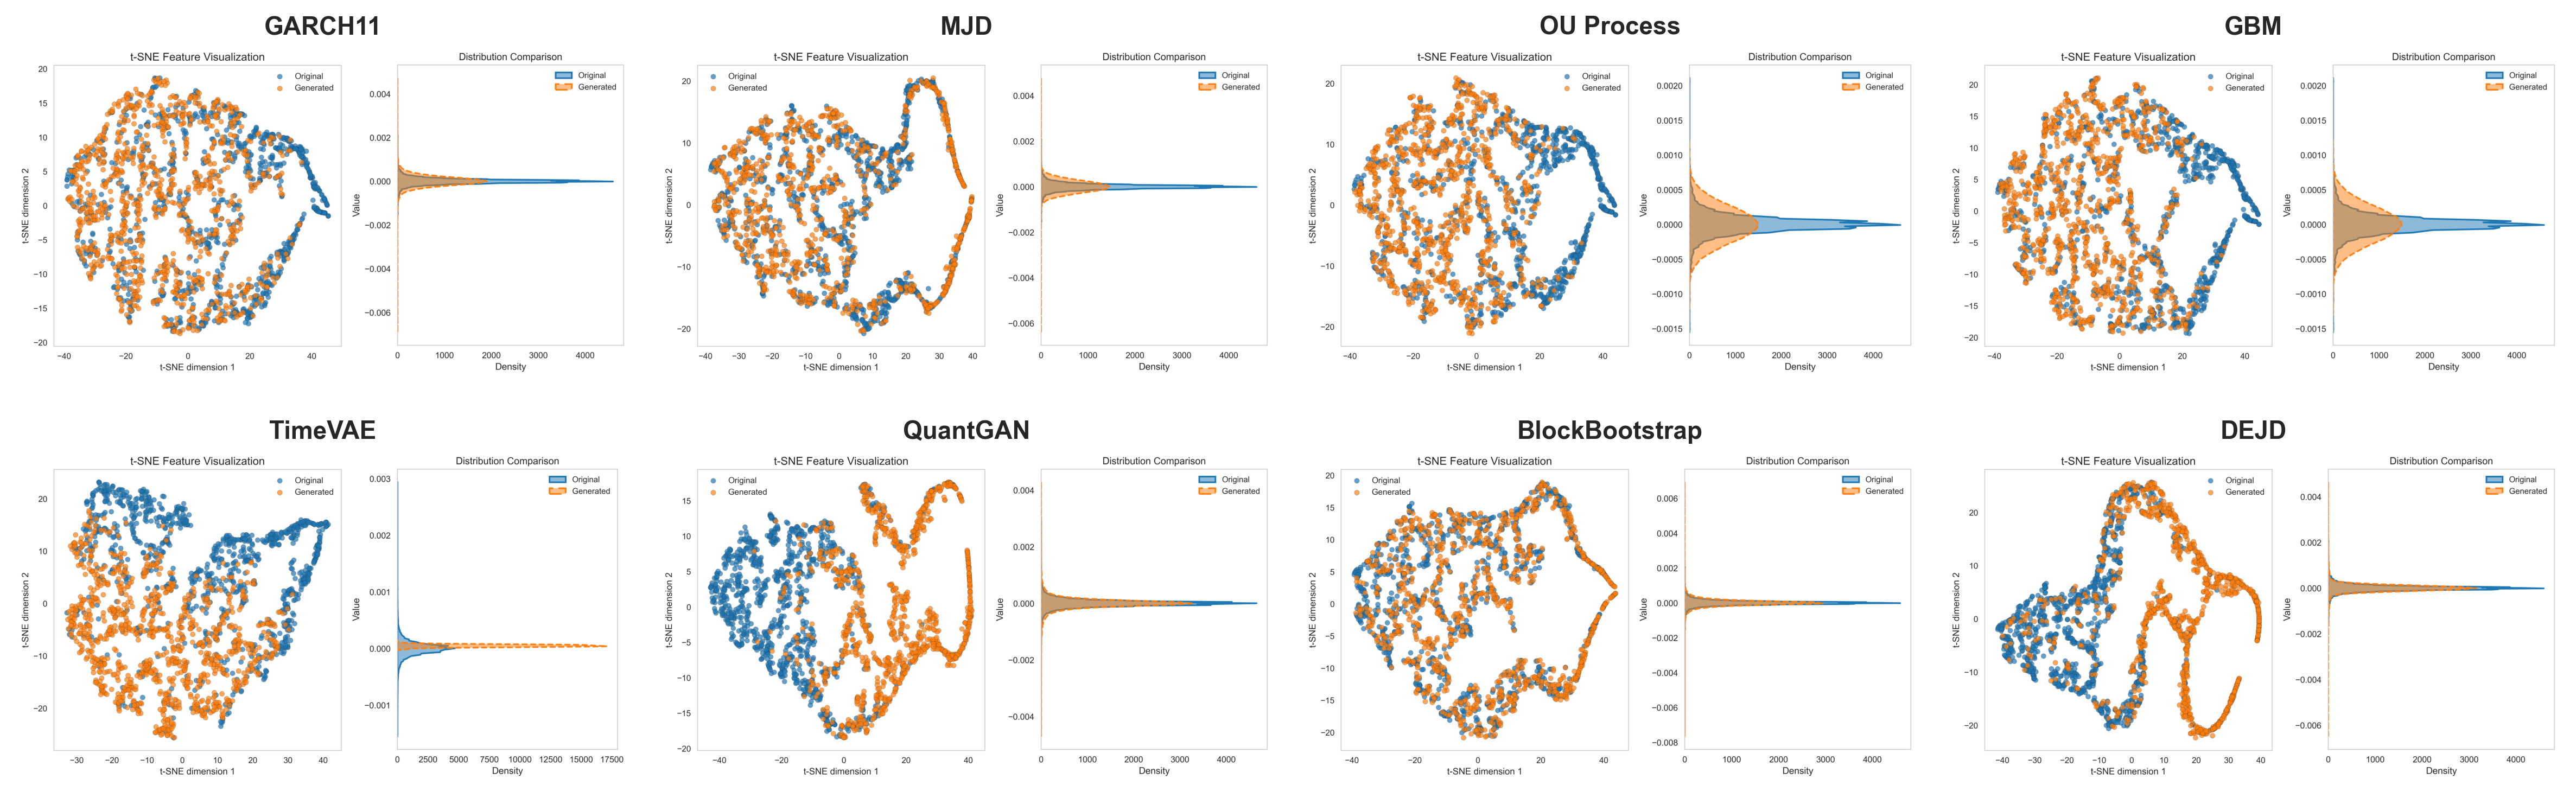
\includegraphics[width=\textwidth,height=8cm,keepaspectratio]
      {../../results/main_experiment/figure_2_tsne_distribution/figure_2_tsne_distribution.png}
      \caption{t-SNE visualization and distribution plots comparing real and synthetic financial time series data across models.
      (Specification: sequence length based on
      maximum significant PACF lag)}
      \Description{t-SNE embeddings and histograms showing the overlap and distributional properties of real versus synthetic data generated by different SDGFTS models.}
      \label{fig:tsne_distribution}
  \end{figure*}

  \subsection{Statistical Evaluation Results}\label{sec:stats_results}
    The following 2 sections are basesd on the results summarized in
    figure \ref{fig:heatmap_all_taxonomies}.
    \subsubsection{Stylized Facts and Fidelity}
    The block bootstrap \ref{alg:blockbootstrap2} consistently 
    achieves the strongest 
    performance across both distributional metrics and stylized facts. 
    This outcome is expected: by resampling contiguous blocks from the 
    training data, the block bootstrap directly inherits empirical 
    marginal distributions \ref{metric:mdd} and short- to 
    medium-range dependence 
    structures. As a result, it naturally preserves key stylized facts 
    (e.g., heavy tails \ref{metric:kd}, volatility clustering 
    \ref{metric:volclustering}) as long as they are present within 
    the chosen block length.

    Among parametric models, GARCH \ref{alg:garch} performs second 
    best overall. This is
    consistent with its widespread use in financial time series modeling:
    GARCH is explicitly designed to capture volatility clustering and
    volatility persistence. While standard GARCH models do not exhibit
    true long-memory behavior (in the strict statistical sense), they
    nonetheless approximate slowly decaying volatility autocorrelations
    well enough to score favorably on stylized-fact metrics relative to
    simpler parametric models such as OU process and GBM.

    The DEJD \ref{alg:dejd} model underperforms on kurtosis-
    based metrics \ref{metric:kd} despite its ability to generate fat tails.
    Although the jump component introduces excess kurtosis relative to pure
    diffusion processes, the model is not inherently calibrated to
    reproduce empirical tail thickness precisely. Its weaker performance
    likely reflects limitations in parameter estimation and
    mismatch between assumed jump dynamics and the empirical return
    distribution.

    Volatility models such as GBM \ref{alg:gbm} and the OU process \ref{alg:ou}
     perform poorly on
    stylized facts (§ \ref{sec:stylized-facts}). This result is unsurprising: 
    both models assume
    conditionally Gaussian increments with constant (GBM) or mean-reverting
    (OU) volatility, and therefore cannot reproduce volatility clustering
    or persistent heteroskedasticity observed in real financial time
    series.

    A notable result is that QuantGAN performs significantly worse on
    distributional metrics while capturing stylized facts relatively well.
    This suggests that the adversarial objective is effective at matching
    temporal dependence and higher-order dynamics, but less effective at
    aligning marginal distributions without explicit distributional
    constraints. TimeVAE performs poorly overall, which is consistent with
    posterior collapse when trained on log returns—limiting its ability to
    generate meaningful variability and capture higher-order financial
    structure.

    \subsubsection{Efficiency}

    Efficiency results largely follow model complexity. GBM, as the
    simplest model both conceptually and computationally, is the fastest
    to train and sample from. In contrast, QuantGAN is the slowest by
    design, reflecting the cost of adversarial training and high-capacity
    neural architectures.

    \subsubsection{Visualization}

    Figure \ref{fig:tsne_distribution} presents t-SNE embeddings and
    return distribution plots (see §\ref{sec:visualization_methods}) 
    for real versus synthetic data across
    models. The block bootstrap \ref{alg:blockbootstrap2}shows 
    near-perfect overlap in t-SNE space, reflecting its direct 
    resampling from real data. QuantGAN \ref{alg:quantgan} and
    DEJD \ref{alg:dejd} also shows better distribution alignment,
    but does not full capture the clusters in the t-SNE plots.

    While other parametric models do not capture these clusters fully,
    they generally corroborate the quantitative findings: GARCH
    \ref{alg:garch} shows better distributional alignment than GBM
    \ref{alg:gbm} and OU process \ref{alg:ou}, while TimeVAE
    \ref{alg:timevae} exhibits the worst overlap and distributional
    mismatch, as it appears to suffer from posterior collapse.

    \subsubsection{Diveristy metrics}\label{sec:diversity_introduce}

    Diversity alone is ambiguous: high variability does not guarantee
    realism and may violate structural dependencies. We therefore evaluate
    diversity jointly with fidelity to ensure variability remains
    plausible. We revisit this in research question \ref{rq:2} and in
    §\ref{sec:metric_tradeoffs}.
    
    \subsection{Utility Evaluation Results}\label{sec:hedger_results}
    \begin{figure*}[h]
      \centering
      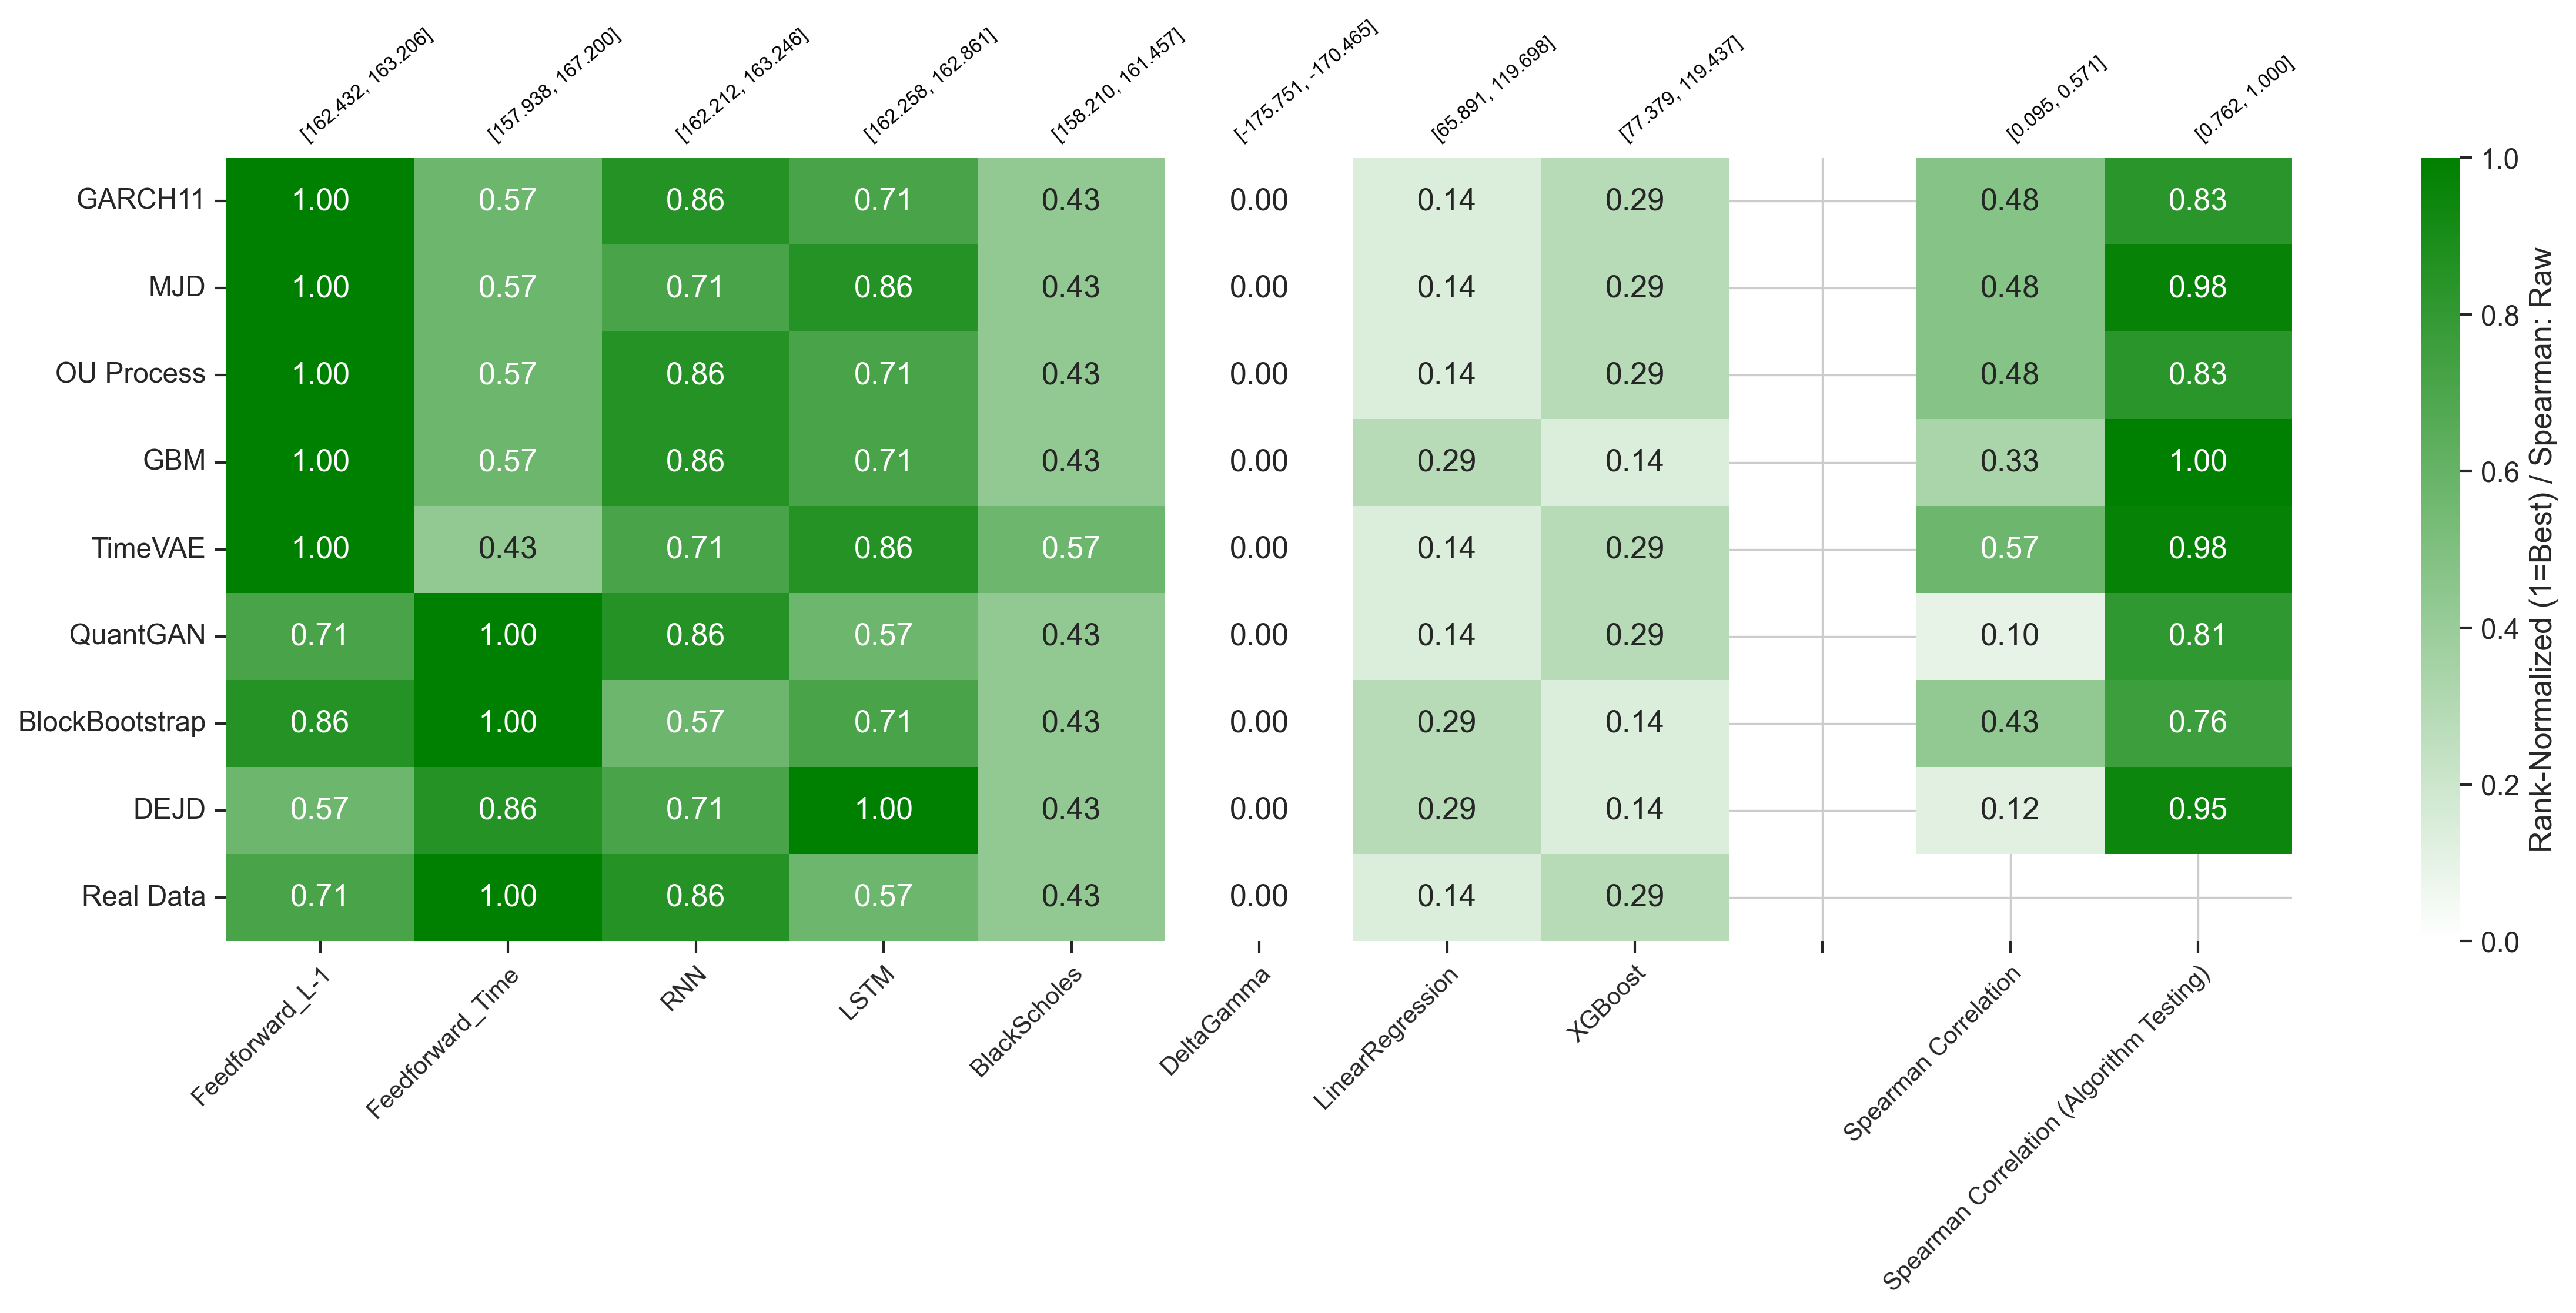
\includegraphics[width=\textwidth,height=8cm,keepaspectratio]
      {../../results/main_experiment/figure_1_per_metric_heatmaps/figure_1_utility_and_algorithm_ranknorm_heatmap.png}
      \caption{Normalized ranking heatmap for mean replication values
      of each hedger trained on SDGFTS/real data. Raw minimum and 
      maximum values are provided for each metric column.
     (Specification: Augmented datasets and sequence length based on
      maximum significant PACF lag).}
      \Description{Heatmap displaying normalized utility metric rankings 
      and algorithm comparison results across different SDGFTS models.}
      \label{fig:heatmap_utility_algorithm}
    \end{figure*}

    As see in Figure \ref{fig:heatmap_utility_algorithm},
    for the augmented testing \ref{sec:augmented-testing}, we can make the observation that for the
    hedging models, the neural network models generally perform better
    than the parametric models in estimating the deltas. This is expected
    as the neural network models are able to capture the higher-order
    dynamics of the index series, which the parametric models are not
    able to capture \cite{Fecamp20}.

    In the augmented-testing setting, with algorithms compared across
    datasets (see §\ref{sec:algorithm-comparison}), we observe that
    the rank-normalized values of the
    heatmaps obtained using QuantGAN \ref{alg:quantgan}
    and BlockBootstrap \ref{alg:blockbootstrap2}
     remain highly consistent with those derived from real-only
    data. In particular, rank-normalized hedging performance under
    QuantGAN augmentation closely matches the baseline ordering, while
    BlockBootstrap augmentation yields nearly identical results. This
    behavior is expected for BlockBootstrap, which preserves empirical
    dependence structures by construction, and suggests that
    QuantGAN-generated samples do not distort the hedger-relevant
    dynamics when mixed with real data. Thus, both augmentation
    strategies maintain the relative sensitivities and preferences of
    hedger models observed under real-data training, indicating that
    these synthetic generators can be used for augmentation without
    materially altering hedging-based performance assessments.

    For Spearman correlation (see Equation \ref{eq:Spearman}),
    recommended by Stenger et al., it's important to note that this metric
    considers only the ranking of model performances, completely ignoring
    the actual delta values between them \cite{Stenger24}. This can be 
    problematic: for
    example, TimeVAE \ref{alg:timevae} \textemdash despite suffering 
    from mode collapse and generating
    less realistic outputs \textemdash may still achieve a high Spearman correlation
    if it preserves the order of model performances, even though the
    deltas may be substantially off or meaningless. Conversely, QuantGAN,
    which better captures the structure of financial data, might produce
    more realistic values but achieve a worse Spearman score if the
    ranking changes slightly. Thus, relying solely on Spearman
    correlation can be misleading, as it overlooks the magnitude and
    quality of differences between models and may obscure meaningful
    distinctions in model performance.
  
  \subsection{\ref{rq:1} Metric Response on Sequence Length Training}
    We investigate how training sequence length affects evaluation
    metrics as posed in research question \ref{rq:1}.
    As previous sections describe how sequence length is determined
    based on model-specific PACF analysis (§\ref{sec:model-specific})
    how they affect the Stonk Bench architecture.

    Recall that the sequence lengths considered are 60, 120, 180, 240,
    and 300 minutes respectively.

  We analyze each metric as the training sequence length varies from
  60 to 300 minutes.

\subsubsection{Fidelity}
  Rank-normalized MDD values are essentially invariant to sequence
  length, which is expected for a marginal distribution metric unless
  models generate time-varying distributions (not observed here).
  Skewness differences show minimal variation for GARCH(1,1), GBM, OU,
  and MJD, suggesting limited sensitivity to sequence length. Modest
  rank improvements for BlockBootstrap and DEJD likely reflect better
  capture of asymmetric tail events. Kurtosis differences for GARCH,
  MJD, OU, and GBM change marginally with sequence length, consistent
  with limited extreme-tail generation; BlockBootstrap improves with
  longer sequences by resampling rare extremes. See the fidelity
  ablation heatmap in Figure~\ref{fig:ablation_fidelity}.

\subsubsection{Diversity}
  Diversity rankings remain stable across sequence lengths, consistent
  with largely unchanged marginal distributions. However, the minimum
  and maximum diversity values increase with sequence length, as longer
  windows permit greater variability across time steps. See the
  diversity ablation heatmap in Figure~\ref{fig:ablation_diversity}.

\subsubsection{Efficiency}
  Maximum generation time increases monotonically with sequence length,
  while model rankings remain unchanged, reflecting computational
  complexity rather than algorithmic reordering. See the efficiency
  ablation heatmap in Figure~\ref{fig:ablation_efficiency}.

\subsubsection{Stylized facts}
  The maximum values for lag-1 autocorrelation of absolute returns and
  volatility clustering increase with sequence length, whereas long
  memory measures tend to decrease. Rankings for QuantGAN,
  BlockBootstrap, and DEJD are largely preserved across lengths. See
  the stylized-facts ablation heatmap in
  Figure~\ref{fig:ablation_stylized_facts}.

\subsubsection{Spearman correlation}
  Spearman's rank correlation summarizes ordering only and can be
  misleading when magnitude differences matter; reliance on it alone is
  therefore discouraged. See the utility correlation comparison in
  Figure~\ref{fig:ablation_utility_spearman}.


  \subsection{\ref{rq:2} Metric Tradeoffs and Interactions}
  \label{sec:metric_tradeoffs}
    We dedicate this subsection to answer the research question
    \ref{rq:2} regarding trade-offs and interactions between different
    evaluation metrics.

    \subsubsection{Diversity versus Fidelity}
      As introduced in §\ref{sec:diversity_introduce}, diversity
      metrics must be interpreted in conjunction with fidelity and
      stylized-fact metrics. How should we interpret these relationships? 
      Recall that "difference" here means the discrepancy between real 
      and synthetic data—the lower the value, the better the model is 
      matching the real data.

      The MDD \ref{metric:mdd} and SDD \ref{metric:sdd} 
      both show a notably strong positive correlation with ICD 
      Euclidean diversity \ref{metric:ed}. For example, MDD has a 
      Pearson correlation coefficient of \( r = 0.68 \) (p = 0.09), 
      and STD difference has an even higher \( r = 0.97 \) 
      (p = 1.90e-4) (see Figure \ref{fig:eclidian_fidelity_diversity}). 
      This indicates that as the marginal or standard deviation 
      difference between real and synthetic data increases (i.e., as 
      fidelity to the real data worsens), the diversity, as measured 
      by ICD Euclidean, also tends to increase.

      The findings indicate that increased diversity, as measured by ICD 
      Euclidean, often correlates with reduced fidelity in basic 
      distributional statistics. This suggests that models generating 
      more diverse samples may deviate significantly from the real data 
      distribution, highlighting the necessity of balancing diversity 
      with fidelity. While some diversity is beneficial for generative 
      models, excessive diversity can lead to less realistic outputs. 
      Therefore, it is crucial to evaluate both fidelity and diversity 
      metrics together when assessing generative time series models.

    \subsubsection{Diversity versus Stylized Facts}
      Figure \ref{fig:eclidian_stylized_facts_diversity} presents
      scatter plots illustrating the relationship between ICD Euclidean
      diversity \ref{metric:ed} and key stylized-fact metrics:
      ACD \ref{metric:acd}, volatility clustering \ref{metric:volclustering},
      and LMSD \ref{metric:slow_decay}.

      Volatility clustering shows a weak positive correlation with
      diversity (p \( \approx \) 0.1). This suggests that more diverse models
      tend to preserve stronger volatility clustering, indicating
      that allowing a broader range of sample paths may help retain
      persistent volatility dynamics, though the evidence is
      marginal.

      Long memory in volatility is also positively and mildly
      correlated with diversity. This implies that models producing
      more varied samples are more likely to exhibit persistent,
      slowly decaying volatility correlations, consistent with
      richer temporal dynamics emerging from increased generative
      flexibility.

    \begin{figure}[h]
      \centering
      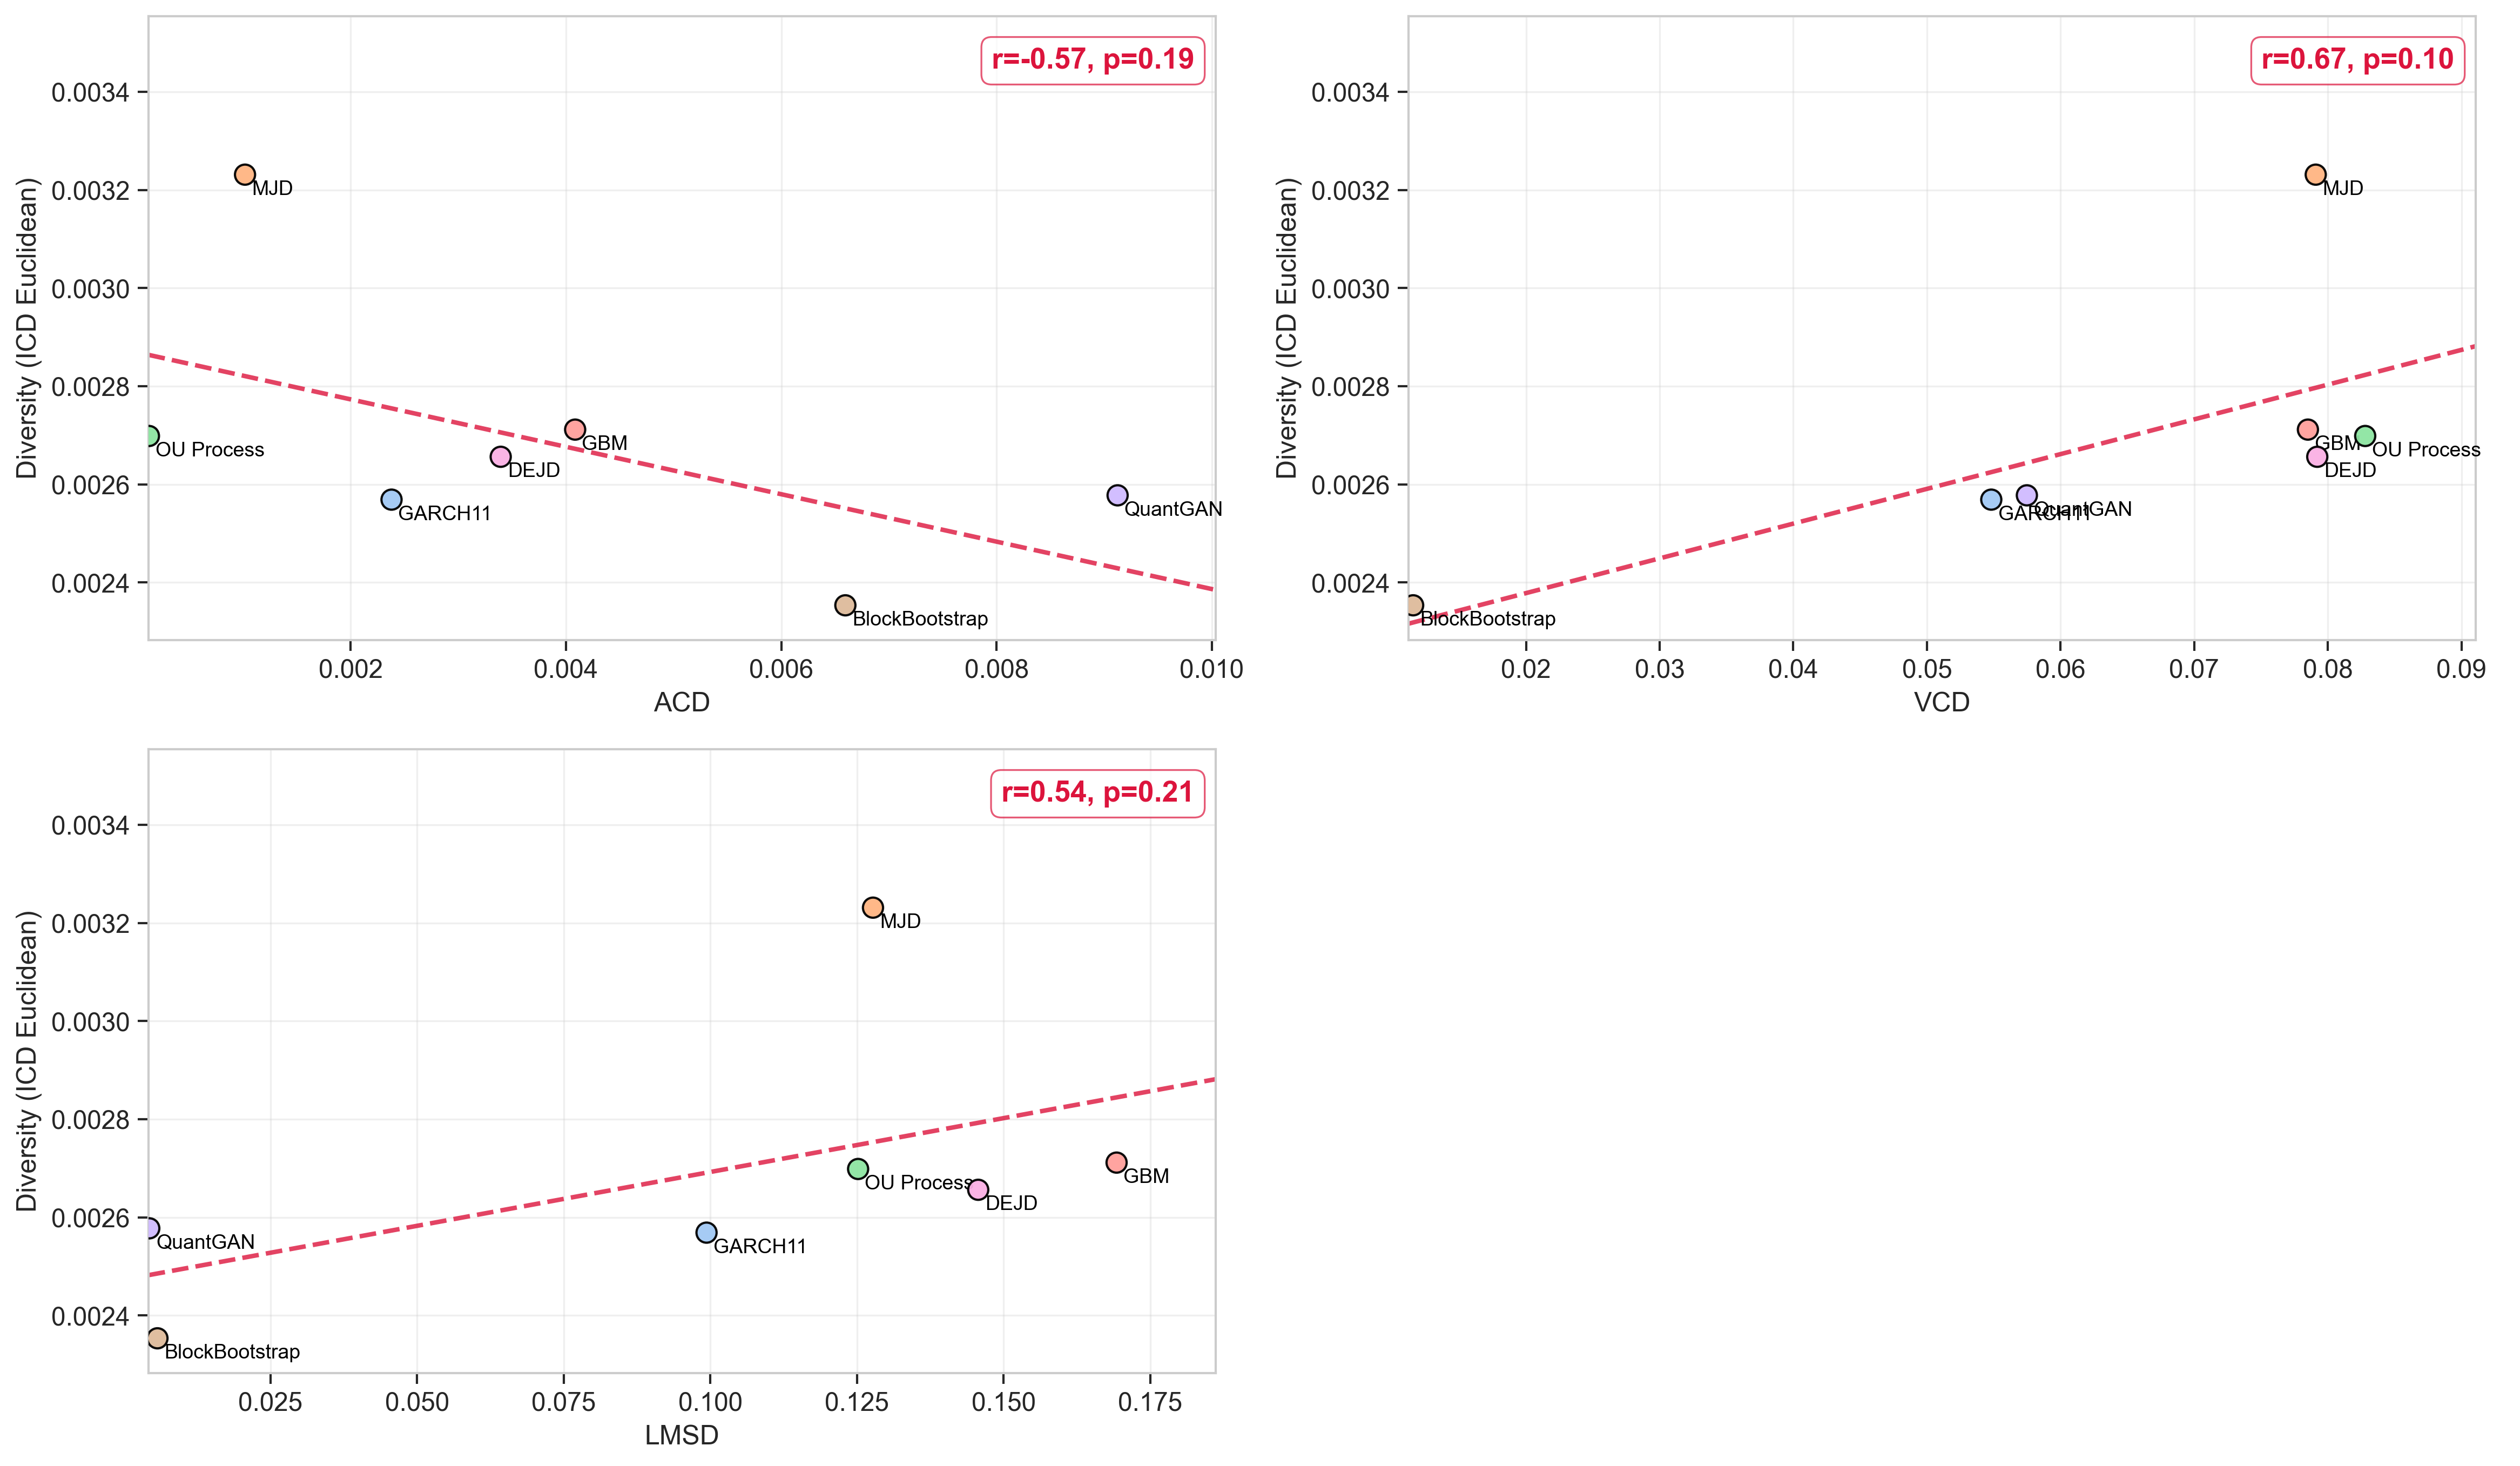
\includegraphics[width=0.45\textwidth,height=6cm,keepaspectratio]
      {../../results/appendix/figure_6_stylized_facts_vs_diversity/figure_6_icd_euclidean_2x2_grid.png}
      \caption{Scatter plots showing the relationship between 
      ICD Euclidean diversity and stylized facts metrics (ACD, 
      volatility clustering, and LMSD). Each point represents a model, 
      with trend lines indicating correlation direction and strength.}
      \Description{Scatter plots illustrating the correlation between 
      ICD Euclidean diversity and stylized facts metrics (ACD, 
      volatility clustering, and LMSD)
      across different models.}
      \label{fig:eclidian_stylized_facts_diversity}
    \end{figure}

    \subsubsection{Efficiency versus other metrics}
      Efficiency, measured by generation time, shows no significant
      correlation with fidelity, diversity, or stylized-fact metrics.
      This indicates that faster models do not necessarily compromise
      on quality or realism, nor do slower models guarantee better
      performance. Thus, efficiency appears to be largely independent
      of other evaluation dimensions in this benchmark.

